\subsection{Package}

Un \textbf{package} è un costrutto che permette di raggruppare un insieme di elementi UML in unità di livello più alto. In genere, si utilizzano per raggruppare classi. Ogni classe fa parte di un solo package, e un package può essere membro di un altro package.

A livello di programmazione, i package UML corrispondono a costrutti di raggruppamento quali gli omonimi \textit{package} di Java o i \textit{namespace} in C++. Ogni package introduce uno \textbf{spazio di nomi} (\textit{namespace}): classi differenti membri dello stesso package devono avere nomi distinti.

I package sono rappresentati graficamente come dei box dotati di linguetta (\textit{tab}) in alto a sinistra. Il nome del package può essere riportato all’interno del box o sul tab se si illustrano i contenuti interni.

\begin{figure}[H]
    \centering
    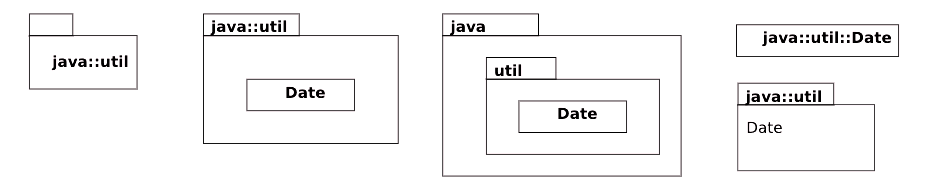
\includegraphics[width=0.75\linewidth]{assets/UML/package/package-1.png}
    \caption{Esempio di rappresentazione di un package UML}
\end{figure}

\paragraph{Classi pubbliche e private}
Le classi contenute in un package UML possono essere \textbf{pubbliche} o \textbf{private}. Le classi pubbliche costituiscono l’interfaccia del package e possono essere utilizzate all’esterno di esso. Per ridurre l’interfaccia di un package, si può esportare solo un sottoinsieme delle operazioni delle classi (\textit{pattern Facade}):
\begin{itemize}
    \item Si dichiarano private tutte le classi;
    \item Si introducono solo poche classi pubbliche che rendono visibile l’interfaccia desiderata.
\end{itemize}

\paragraph{Principi di suddivisione di classi in package}
La suddivisione delle classi in package dovrebbe seguire i seguenti principi:
\begin{itemize}
    \item \textbf{Common Closure}: le classi dello stesso package dovrebbero condividere le cause di un eventuale cambiamento.
    \item \textbf{Common Reuse}: le classi dello stesso package dovrebbero essere riusate insieme.
\end{itemize}

\subsubsection{Package e dipendenze}
Un \textbf{diagramma dei package} documenta i package e le dipendenze tra di essi. Le dipendenze tra package riassumono quelle tra gli elementi contenuti. Un diagramma generale dei package è utile per tenere sotto controllo la complessità strutturale del codice.

Man mano che le dipendenze entranti in un package aumentano, la sua interfaccia deve essere sempre più stabile (\textit{Dependencies principle}). I package più stabili tendono a contenere una percentuale maggiore di classi astratte e interfacce (\textit{Stable abstraction principle}).

\begin{figure}[H]
    \centering
    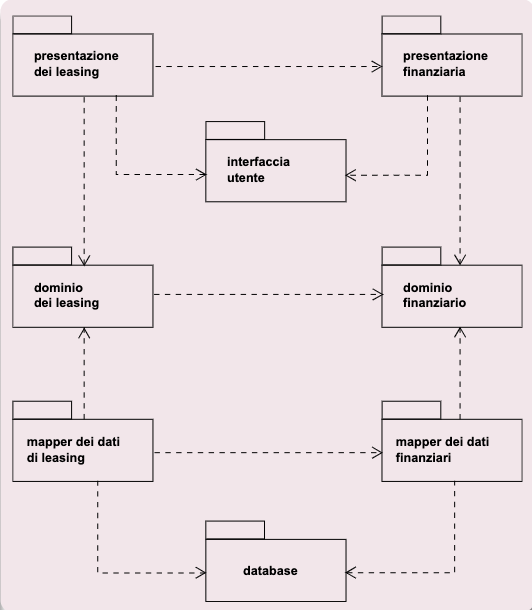
\includegraphics[width=0.75\linewidth]{assets/UML/package/package-2.png}
    \caption{Esempio di dipendenze tra package}
\end{figure}

\subsubsection{Dipendenze \textit{access} e \textit{import}}
Entrambe le parole chiave sono utilizzate per indicare che un package include nel proprio \textit{namespace} i nomi definiti in un altro package:
\begin{itemize}
    \item La parola chiave \textbf{\textit{import}} indica un’importazione di tipo \textbf{public}: gli elementi importati sono aggiunti al \textit{namespace} e resi visibili anche all’esterno.
    \item La parola chiave \textbf{\textit{access}} indica un’importazione di tipo \textbf{private}: gli elementi importati sono aggiunti al \textit{namespace} ma non sono visibili dall’esterno.
\end{itemize}

\begin{figure}[H]
    \centering
    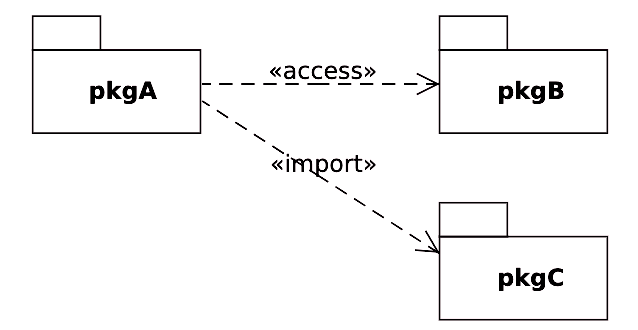
\includegraphics[width=0.75\linewidth]{assets/UML/package/package-3.png}
    \caption{Esempio di dipendenze \textit{access} e \textit{import}}
\end{figure}

\subsubsection{Gerarchia di package}
La gerarchia dei package può essere visualizzata tramite una struttura ad albero. Ogni nodo rappresenta un package e i suoi sottopackage.

\begin{figure}[H]
    \centering
    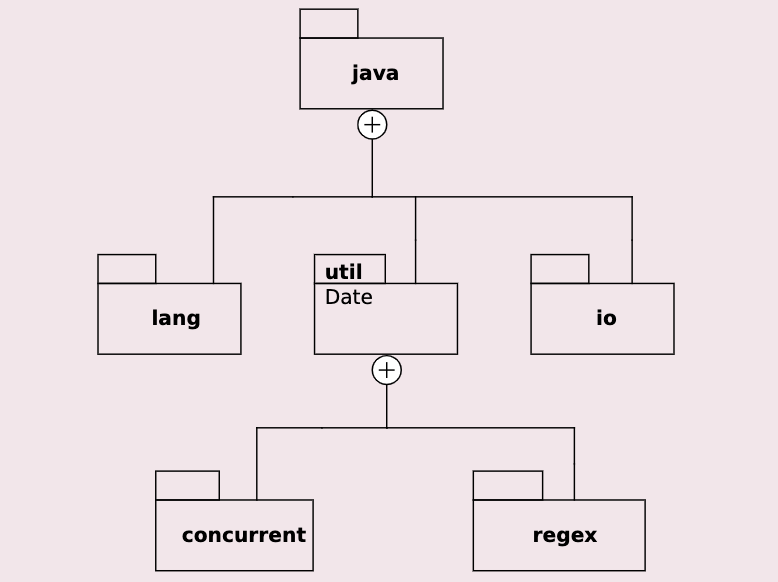
\includegraphics[width=0.75\linewidth]{assets/UML/package/package-4.png}
    \caption{Esempio di gerarchia di package}
\end{figure}

\newpage